\subsection{Search Tree}
    \begin{itemize}
        \item sorted data
        \item all operations fast
        \item well organized
    \end{itemize}
    \subsubsection{Tree terminology} \label{sec_tree_terminology}
        \begin{itemize}
            \item Root: Highest node has children and no parent
            \item Order: Maximum number of child nodes (BST order = 2)
            \item Height: Maximum path length root to leaf
            \item Degenerated: Every Node has only one child, leading to a linked list structure
            \item Complete: Every level except for the lowest is filled, lowest level is filled from left to right
            \item Perfect: Every level is completely filled
            \item Full: the amount of children of every node equals either the order or 0
            \item ALV-Tree: balanced binary search tree ($-1 \leq \text{height(n.left)} - \text{height(n.right)} \leq 1)$
        \end{itemize}
    
    \subsubsection{Binary Tree Traversal}
        {\centering\underline{\textbf{Preorder}} \par}
            \begin{minipage}{0.49\linewidth}
                \lstinputlisting{src/4_data_structure/code/preorder.py}
                If a list 'a' was the inorder traversal of a tree: the tree can always be recreated\\
                $\Rightarrow$ \textbf{Representation unique}
            \end{minipage}
            \begin{minipage}{0.49\linewidth}
                {\centering 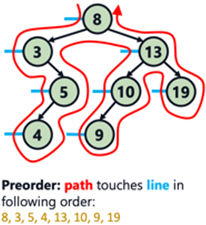
\includegraphics[width = 0.85\linewidth]{src/4_data_structure/images/preorder.png} \par}
            \end{minipage}

        {\centering\underline{\textbf{Inorder}} \par}
            \begin{minipage}{0.49\linewidth}
                \lstinputlisting{src/4_data_structure/code/inorder.py}
                Entries are printed in ascending order\\
                If a list 'a' was the inorder traversal of a tree: the tree can be recreated only if the list is in ascending order\\
                $\Rightarrow$ \textbf{Representation not unique}
            \end{minipage}
            \begin{minipage}{0.49\linewidth}
                {\centering 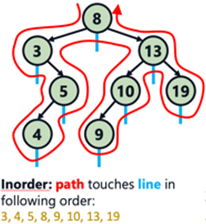
\includegraphics[width = 0.85\linewidth]{src/4_data_structure/images/inorder.png} \par}
            \end{minipage}

        {\centering\underline{\textbf{Postorder}} \par}
            \begin{minipage}{0.49\linewidth}
                \lstinputlisting{src/4_data_structure/code/postorder.py}
                If a list 'a' was the inorder traversal of a tree: the tree can always be recreated\\
                $\Rightarrow$ \textbf{Representation unique}
            \end{minipage}
            \begin{minipage}{0.49\linewidth}
                {\centering 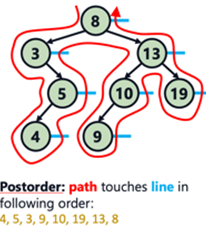
\includegraphics[width = 0.85\linewidth]{src/4_data_structure/images/postorder.png} \par}
            \end{minipage}


    \subsubsection{Binary Search Tree (BST)}
        \begin{minipage}{0.49\linewidth}
            A binary search tree is a binary tree which fulfils the following:
            \begin{enumerate}
                \item Every node v stores a key
                \item Keys in the left subtree are smaller than v.key
                \item Keys in the right subtree are larger than v.key
            \end{enumerate}
        \end{minipage}
        \begin{minipage}{0.49\linewidth}
            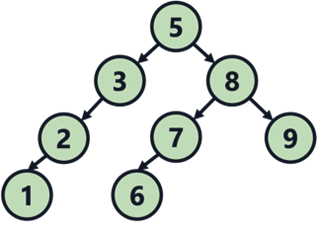
\includegraphics[width = \linewidth]{src/4_data_structure/images/bst.png}
        \end{minipage}

        {\centering\underline{\textbf{Implementation}} \par}
            \lstinputlisting{src/4_data_structure/code/bst_implementation.py}

        {\centering\underline{\textbf{Height}} \par}
            \lstinputlisting{src/4_data_structure/code/bst_height.py}

        {\centering\underline{\textbf{Search for Node}} \par}
            \lstinputlisting{src/4_data_structure/code/bst_search.py}

        {\centering\underline{\textbf{Insert Node}} \par}
            \lstinputlisting{src/4_data_structure/code/bst_insert.py}

        {\centering\underline{\textbf{Remove Node}} \par}
            \begin{minipage}{0.49\linewidth}
                Cases:
                \begin{enumerate}
                    \item node has no children: set variable to None
                    \item node has one child: replace node with child
                    \item node has two children: replace node with symmetric successor – the next biggest element
                \end{enumerate}
            \end{minipage}
            \begin{minipage}{0.49\linewidth}
                Case 3:\\
                \includegraphics*[width = \linewidth]{src/4_data_structure/images/symmetric_successor.png}
            \end{minipage}

            \lstinputlisting{src/4_data_structure/code/bst_remove.py}